\lecture{Security}{11:00}{14/10/24}{Asim Ali}

\section*{Security Factors}

There are three main security factors we need to consider--
\begin{itemize}
  \item Confidentiality
  \begin{itemize}
    \item Only authorised parties should be able to read the information
  \end{itemize}
  \item Integrity
  \begin{itemize}
    \item Only authorised parties should be able to modify, create and delete information
  \end{itemize}
  \item Availability
  \begin{itemize}
    \item Authorised parties should always have access to the information
  \end{itemize}
\end{itemize}

\section*{Types of Attackers}

\begin{itemize}
  \item Passive Attackers
  \begin{itemize}
    \item The attacker only listens to the messages, so they can only read the information
  \end{itemize}
  \item Active Attackers
  \begin{itemize}
    \item The attacker listens, modifies and sends messages, so they can read the information, modify it or fabricate
     it entirely
  \end{itemize}
\end{itemize}

To overcome both of these types of attacker, you can encrypt the data, meaning that it is unreadable by any third parties,
 and if someone attempts to modify or spoof a message, it will not be encrypted with the same key and so the receiver
 will know it was not sent by the correct person.

\section*{Symmetric (Shared Key) Encryption}

Symmetric key encryption requires the sender and receiver to already have a shared key, which will then be used to both
 encrypt and decrypt the messages.

\subsection*{DES (Data Encryption Standard)}

Plaintext is split into 64-bit blocks. The key is 56-bits long and 16 subkeys are generated for 16 rounds of cryptography.
 The subkeys are then used in reverse order to decrypt the data. Because this quickly became insecure, Triple-DES was
 created as a new standard, which is as literal as the name suggests. You simply encrypt the data three times with
 three different keys, then decrypt 3 times in reverse order.

\subsection*{AES (Advanced Encryption Standard)}

Plaintext is split into 128-bit blocks. The key is 128,192 or 256-bits long, giving the algorithm the name AES-128/192/256.
 AES is a much more advanced algorithm than DES, and it was created with the express purpose of replacing DES

\subsection*{Confidentiality}

Because the messages are encrypted, they cannot be read or examined by a third party. This does rely upon the keys being
 shared ahead of time, in a secure way such that no third parties know what the key is.

\section*{Asymmetric (Public Key) Encryption}

In asymmetric encryption, the sender and receiver have two different but related keys. The sender uses the public key of
 the receiver to encrypt the message, and the receiver uses their own private key to decrypt the message.

\subsection*{RSA (Rivest-Shamir-Adleman)}

\begin{enumerate}
  \item Select two large primes $p$ and $q$ (the larger the better)
  \item $n = pq$ and $z = (p - 1)(q - 1)$
  \item Select a number relatively prime (such that they have no common divisors) to $z$ and call it $d$
  \item Find $e$ such that $e * d = 1 \mod z$
  \item The public key is then $(e, n)$ and the private key $(d, n)$
  \item To encrypt a message, convert the plaintext $M$ into an integer $m$ such that $0 \leq m < n$, using a known
   and reversible padding scheme. Then compute the ciphertext $c$ such as $c = m^e (\mod n)$
  \item To then decrypt the message, you use the private key $d$ by computing $c^d = {(m^e)}^d = m (\mod n)$. Then given
   $m$, you recover the message $M$ by reversing the padding scheme
\end{enumerate}

\begin{figure}[h]
  \caption{Encrypt then decrypt the string `PORT' with the public key $(3, 33)$ and the private key $(7, 33)$}
  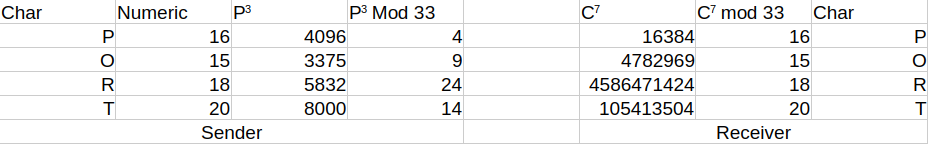
\includegraphics[width=0.9\linewidth]{assets/lect3-ex1.png}
  \centering
\end{figure}

\subsection*{Confidentiality}

Because the messages are encrypted, they cannot be read or examined by a third party. Since the public key can only be
 used to encrypt messages (theoretically it can be used to determine the private key but this is effectively impossible
 with current computational power), it can be sent out on the internet for anyone to use to encrypt messages for the
 receiver. As long as the private key is kept secret by the receiver, the messages are perfectly confidential.

\section*{Ensuring Integrity}

To make sure that a message was sent by the correct person, and without being modified we can use either signatures,
 message digests or both.

\subsection*{Digital Signatures}

When making a digital signature, the inverse of public-key cryptography is done. This means that only the owner of the
 signature knows the private key, but everyone knows the public key. The private key is used to cryptographically sign
 a file or message, which anyone can use the public key to verify, but only the owner of the keypair can use their key
 to sign. This means that if a message is signed, it must've come from the correct person.

\subsection*{Message Digests}

A message digest (or hash function) takes a message $M$ and produces a small `fingerprint' known as the message digest
 $H(M)$. A secure hash function $H$ encrypts a small block of the message which is produced as a function of the message,
 known as the authenticator. The properties of $H$ are such that $H(M) \neq H(M')$ and given $H(M)$ is is computationally
 impossible to find $M$. The message digest is encrypted with the sender's private key, and serves as a signature that
 verifies the content and order of the message. Two popular digest functions are MD5 and SHA-1.

\section*{Authentication}

Authentication verifies that a message has come from a verified source. This can be achieved using conventional encryption
 techniques as discussed previously. This does not protect against so-called playback attacks however. If a third party
 records an encrypted message, they can re-send it again at a later time, and since the message is correctly encrypted,
 the receiver will still believe it to be a valid message.

This can be avoided by adding a number to the cipher that relates to the time the message was sent, either directly or
 by using it as the seed for a random number generator. When the message is received, if the time is too far in the
 past, the message will either be ignored, or requested for re-sending to ensure the correct message was sent.